\documentclass[aspectratio=169]{beamer}

% ── Theme ──────────────────────────────────────────────────────────────────────
\usetheme{Madrid}
\usecolortheme{whale}
\usefonttheme{serif}
\setbeamertemplate{navigation symbols}{}
\setbeamertemplate{headline}{}
\setbeamertemplate{footline}{%
  \leavevmode\hbox{%
    \begin{beamercolorbox}[wd=.33\paperwidth,ht=2.25ex,dp=1ex,center]{author in head/foot}%
      \usebeamerfont{author in head/foot}\insertshortauthor
    \end{beamercolorbox}%
    \begin{beamercolorbox}[wd=.34\paperwidth,ht=2.25ex,dp=1ex,center]{title in head/foot}%
      \usebeamerfont{title in head/foot}\insertshorttitle
    \end{beamercolorbox}%
    \begin{beamercolorbox}[wd=.33\paperwidth,ht=2.25ex,dp=1ex,right]{date in head/foot}%
      \usebeamerfont{date in head/foot}\insertframenumber{} / \inserttotalframenumber\hspace*{1.5ex}
    \end{beamercolorbox}%
  }\vskip0pt%
}

% ── Colours ────────────────────────────────────────────────────────────────────
\definecolor{iitgblue}{RGB}{0,53,107}
\definecolor{iitggold}{RGB}{185,143,45}
\definecolor{lightblue}{RGB}{220,235,250}
\definecolor{lightgold}{RGB}{255,248,220}

\setbeamercolor{frametitle}{bg=iitgblue,fg=white}
\setbeamercolor{title}{fg=white}
\setbeamercolor{author}{fg=white}
\setbeamercolor{institute}{fg=iitggold}
\setbeamercolor{date}{fg=white}
\setbeamercolor{palette primary}{bg=iitgblue,fg=white}
\setbeamercolor{palette secondary}{bg=iitgblue!80,fg=white}
\setbeamercolor{palette tertiary}{bg=iitgblue!60,fg=white}
\setbeamercolor{block title}{bg=iitgblue,fg=white}
\setbeamercolor{block body}{bg=lightblue}
\setbeamercolor{alertblock title}{bg=red!70!black,fg=white}
\setbeamercolor{alertblock body}{bg=red!8}
\setbeamercolor{exampleblock title}{bg=iitggold!80!black,fg=white}
\setbeamercolor{exampleblock body}{bg=lightgold}
\setbeamercolor{section in toc}{fg=iitgblue}
\setbeamercolor{itemize item}{fg=iitgblue}
\setbeamercolor{itemize subitem}{fg=iitggold!80!black}
\setbeamertemplate{itemize item}{\color{iitgblue}$\blacktriangleright$}
\setbeamertemplate{itemize subitem}{\color{iitggold!80!black}$\bullet$}

% ── Packages ───────────────────────────────────────────────────────────────────
\usepackage{graphicx}
\usepackage{amsmath,amssymb,amsfonts}
\usepackage{booktabs}
\usepackage{multirow}
\usepackage{xcolor}
\usepackage{tikz}
\usetikzlibrary{arrows.meta,positioning,shapes.geometric}
\usepackage[T1]{fontenc}
\usepackage[utf8]{inputenc}
\usepackage{lmodern}
\usepackage{microtype}

% ── Meta ───────────────────────────────────────────────────────────────────────
\title[STMN for Video Re-ID]{Video-based Person Re-identification\\[4pt]with Spatial and Temporal Memory Networks}
\subtitle{\small Paper Implementation --- CS699 / DSAI Project}
\author[Pushpendra Singh]{\textbf{Pushpendra Singh}\\{\small Roll No.\ 240150026}}
\institute[DSAI, IIT Guwahati]{%
  Mehta Family School of Data Science and Artificial Intelligence\\
  Indian Institute of Technology, Guwahati}
\date{April 2026}

% ── Helpers ────────────────────────────────────────────────────────────────────
\newcommand{\bt}[1]{\textbf{#1}}
\newcommand{\eq}[1]{\begin{equation*}#1\end{equation*}}

% ══════════════════════════════════════════════════════════════════════════════
\begin{document}
% ══════════════════════════════════════════════════════════════════════════════

% ── Title slide ───────────────────────────────────────────────────────────────
{
\setbeamertemplate{footline}{}
\begin{frame}
  \vspace{0.5em}
  \titlepage
  \vspace{-0.5em}
  \begin{center}
    \textcolor{iitggold}{\rule{0.6\textwidth}{0.6pt}}\\[4pt]
    {\footnotesize Eom, Lee, Lee \& Ham \quad $\cdot$ \quad \href{https://arxiv.org/abs/2108.09039}{arXiv:2108.09039}, 2021}
  \end{center}
\end{frame}
}

% ── Outline ───────────────────────────────────────────────────────────────────
\begin{frame}{Outline}
  \tableofcontents[sectionstyle=show,subsectionstyle=hide]
\end{frame}

% ══════════════════════════════════════════════════════════════════════════════
\section{Introduction \& Motivation}
% ══════════════════════════════════════════════════════════════════════════════

\begin{frame}{What is Person Re-Identification?}
  \begin{block}{Paper}
    \bt{``Video-based Person Re-identification with Spatial and Temporal Memory Networks''}\\
    Eom, Lee, Lee \& Ham \hfill \textit{Yonsei University --- \href{https://arxiv.org/abs/2108.09039}{arXiv:2108.09039}, 2021}
  \end{block}
  \vspace{0.2em}
  \begin{alertblock}{Task Definition}
    Given a \bt{query person} from one camera, automatically find the \bt{same person}\\
    in footage from other cameras with \bt{no overlapping fields of view}.
  \end{alertblock}
  \vspace{0.2em}
  \begin{columns}[T]
    \column{0.48\textwidth}
      \bt{Why is it hard?}
      \begin{itemize}\setlength\itemsep{2pt}
        \item Varying viewpoints and lighting
        \item Clothing changes across days
        \item Background clutter in every frame
        \item Partial occlusions (walls, bikes, people)
      \end{itemize}
    \column{0.48\textwidth}
      \bt{Video-ReID is harder still:}
      \begin{itemize}\setlength\itemsep{2pt}
        \item Sequences share the same background noise across all frames
        \item Occlusion patterns repeat over time
        \item Frame misalignment during fast motion
      \end{itemize}
  \end{columns}
\end{frame}

% ─────────────────────────────────────────────────────────────────────────────
\begin{frame}{Why Existing Methods Fall Short}
  \begin{columns}[T]
    \column{0.48\textwidth}
      \begin{block}{Attention-based (QAN, STA)}
        \footnotesize Assign per-frame attention weights independently. No global sequence view --- can fixate on non-discriminative regions.
      \end{block}
      \vspace{0.2em}
      \begin{block}{Co-attention (GLTR, COSAM)}
        \footnotesize Use non-local / graph networks across frames. Shared background clutter gets \emph{amplified}, not removed.
      \end{block}
      \vspace{0.2em}
      \begin{alertblock}{Shared Weakness}
        \footnotesize None of these methods \bt{model why} certain regions are distracting in the first place.
      \end{alertblock}

    \column{0.48\textwidth}
      \begin{exampleblock}{Key Observation --- STMN}
        \footnotesize
        \begin{enumerate}\setlength\itemsep{2pt}
          \item \bt{Spatial distractors} (trees, lights, pavers) appear at the \bt{same fixed locations} in every frame of a given camera.
          \item \bt{Temporal occlusion patterns} repeat across many sequences (e.g.\ occluded in first 2 frames, or vanishes at the clip end).
        \end{enumerate}
      \end{exampleblock}
      \vspace{0.2em}
      \begin{alertblock}{Core Idea}
        \footnotesize \bt{Store} these recurring patterns in external memory.\\ \bt{Look them up} at test time --- no relearning needed.
      \end{alertblock}
  \end{columns}
\end{frame}

% ══════════════════════════════════════════════════════════════════════════════
\section{Architecture}
% ══════════════════════════════════════════════════════════════════════════════

\begin{frame}{STMN: Overall Pipeline}
  \vspace{0.3em}

  % Pipeline diagram via TikZ
  \begin{center}
  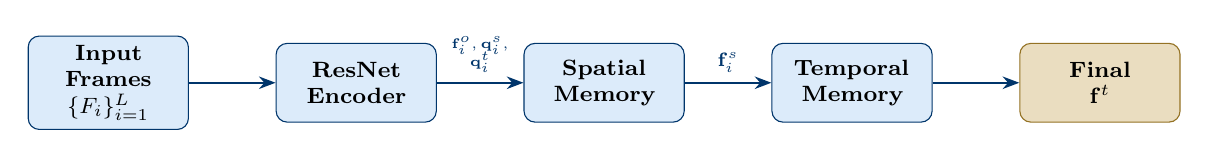
\begin{tikzpicture}[
      node distance = 1.5cm and 1.1cm,
      box/.style    = {draw=iitgblue, fill=lightblue, rounded corners=4pt,
                       minimum height=1cm, text width=1.8cm, align=center,
                       font=\footnotesize\bfseries},
      arr/.style    = {-{Stealth[length=6pt]}, thick, color=iitgblue},
    ]
    \node[box] (frames) {Input Frames $\{F_i\}_{i=1}^{L}$};
    \node[box, right=1.1cm of frames] (enc)    {ResNet\\Encoder};
    \node[box, right=1.1cm of enc]    (sm)     {Spatial\\Memory};
    \node[box, right=1.1cm of sm]     (tm)     {Temporal\\Memory};
    \node[box, right=1.1cm of tm, fill=iitggold!30, draw=iitggold!80!black]
                                       (out)    {Final\\$\mathbf{f}^t$};

    \draw[arr] (frames) -- (enc);
    \draw[arr] (enc)    -- node[above,font=\tiny,align=center]{$\mathbf{f}^o_i,\mathbf{q}^s_i,$\\[-2pt]$\mathbf{q}^t_i$} (sm);
    \draw[arr] (sm)     -- node[above,font=\scriptsize]{$\mathbf{f}^s_i$} (tm);
    \draw[arr] (tm)     -- (out);
  \end{tikzpicture}
  \end{center}

  \vspace{0.5em}
  \bt{Three feature maps produced per frame $i$ (from three separate conv heads):}
  \vspace{0.3em}
  \begin{columns}[T]
    \column{0.30\textwidth}
      \centering
      \colorbox{lightblue}{\parbox{0.9\linewidth}{\centering\small$\mathbf{f}^o_i \in \mathbb{R}^{D \times K}$\\[2pt] Person representation}}
    \column{0.30\textwidth}
      \centering
      \colorbox{lightblue}{\parbox{0.9\linewidth}{\centering\small$\mathbf{q}^s_i \in \mathbb{R}^{D \times K}$\\[2pt] Spatial mem.\ query}}
    \column{0.30\textwidth}
      \centering
      \colorbox{lightblue}{\parbox{0.9\linewidth}{\centering\small$\mathbf{q}^t_i \in \mathbb{R}^{D \times K}$\\[2pt] Temporal mem.\ query}}
  \end{columns}

  \vspace{0.5em}
  \begin{exampleblock}{}
    \small $K = H \times W$ is the number of spatial positions per feature map.\\
    Heads are \bt{separate} --- identity and context features do not share gradients.
  \end{exampleblock}
\end{frame}

% ─────────────────────────────────────────────────────────────────────────────
\begin{frame}{Spatial Memory --- Matching \& Retrieval}
  \vspace{-0.8em}
  \begin{columns}[T]
    \column{0.50\textwidth}
      \footnotesize
      \bt{Key-value store with $M$ slots:}
      \begin{itemize}\setlength\itemsep{0pt}
        \item $\mathbf{k}^s \in \mathbb{R}^{D \times M}$ --- keys
        \item $\mathbf{v}^s \in \mathbb{R}^{D \times M}$ --- distractor patterns
      \end{itemize}

      \bt{Step 1 --- Matching probability} for position $k$, frame $i$, slot $n$:
      \eq{\resizebox{0.8\linewidth}{!}{$\displaystyle
        a^s_{i,k,n} = \frac{\exp\!\bigl((\mathbf{q}^s_{i,k})^\top \mathbf{k}^s_n\bigr)}
                           {\displaystyle\sum_{n'=1}^{M} \exp\!\bigl((\mathbf{q}^s_{i,k})^\top \mathbf{k}^s_{n'}\bigr)}
      $}}

      \bt{Step 2 --- Retrieve distractor feature:}
      \eq{\resizebox{0.6\linewidth}{!}{$\displaystyle \mathbf{o}^s_{i,k} = \sum_{n=1}^{M} a^s_{i,k,n}\; \mathbf{v}^s_n $}}

    \column{0.45\textwidth}
      \footnotesize
      \bt{Step 3 --- Subtract to clean:}
      \eq{\resizebox{0.75\linewidth}{!}{$\displaystyle \mathbf{f}^s_{i,k} = \mathbf{f}^o_{i,k} - \mathrm{BN}\!\left(\mathbf{o}^s_{i,k}\right) $}}

      \begin{alertblock}{Why Batch Norm?}
        \scriptsize Memory output and encoder feature live on very different scales. Without BN the subtraction is dominated by scale mismatch and training diverges completely.
      \end{alertblock}

      \begin{exampleblock}{Intuition}
        \scriptsize $a^s_{i,k,n}$ measures how likely position $k$ contains distractor pattern $n$. We subtract out exactly that distractor, leaving only person features.
      \end{exampleblock}
  \end{columns}
\end{frame}

% ─────────────────────────────────────────────────────────────────────────────
\begin{frame}{Temporal Memory --- Encode, Retrieve, Aggregate}
  \vspace{-0.8em}
  \begin{columns}[T]
    \column{0.48\textwidth}
      \footnotesize
      \bt{Key-value store with $N$ slots:}
      \begin{itemize}\setlength\itemsep{0pt}
        \item $\mathbf{k}^t \in \mathbb{R}^{D \times N}$ --- temporal pattern prototypes
        \item $\mathbf{v}^t \in \mathbb{R}^{L \times N}$ --- stored frame-weight vectors
      \end{itemize}

      \bt{Step 1 --- Encode sequence context via LSTM:}
      \eq{\resizebox{0.8\linewidth}{!}{$\displaystyle
        \mathbf{q}^t = \mathrm{LSTM}\!\Bigl(
          \bigl[\mathrm{GAP}(\mathbf{q}^t_1),\,\ldots,\,\mathrm{GAP}(\mathbf{q}^t_L)\bigr]
        \Bigr)
      $}}
      $\mathbf{q}^t \in \mathbb{R}^D$ = last hidden state\\
      {\scriptsize (encodes pattern like ``occluded in first 2 frames'')}

      \begin{alertblock}{\small Important}
        \scriptsize LSTM only produces the \bt{query context} $\mathbf{q}^t$. It does \emph{not} aggregate features directly.
      \end{alertblock}

    \column{0.48\textwidth}
      \footnotesize
      \bt{Step 2 --- Match context to memory keys:}
      \eq{\resizebox{0.6\linewidth}{!}{$\displaystyle
        a^t_n = \frac{\exp\!\bigl((\mathbf{q}^t)^\top \mathbf{k}^t_n\bigr)}
                    {\displaystyle\sum_{n'=1}^{N} \exp\!\bigl((\mathbf{q}^t)^\top \mathbf{k}^t_{n'}\bigr)}
      $}}
      \bt{Step 3 --- Retrieve frame attention vector:}
      \eq{\resizebox{0.6\linewidth}{!}{$\displaystyle \mathbf{o}^t = \sum_{n=1}^{N} a^t_n\; \mathbf{v}^t_n \;\in \mathbb{R}^{L} $}}

      \bt{Step 4 --- Softmax \& aggregate:}
      \eq{\resizebox{0.6\linewidth}{!}{$\displaystyle
        \mathbf{f}^t = \sum_{i=1}^{L} \hat{o}^t_i \cdot \mathrm{GAP}\!\left(\mathbf{f}^s_i\right)
      $}}
      \begin{exampleblock}{\small Output}
        \scriptsize $\mathbf{f}^t \in \mathbb{R}^D$ --- final identity descriptor.\\
        Low $\hat{o}^t_i$ for occluded frames, high for clear ones.
      \end{exampleblock}
  \end{columns}
\end{frame}

% ══════════════════════════════════════════════════════════════════════════════
\section{Training Strategy}
% ══════════════════════════════════════════════════════════════════════════════

\begin{frame}{Loss 1 --- Memory Spread Loss $\mathcal{L}_S$}
  \vspace{-0.8em}
  \begin{alertblock}{Problem without this loss}
    \footnotesize The model collapses to using 1--2 memory slots for every single input. All other slots become inactive. The memory is effectively useless.
  \end{alertblock}

  \footnotesize
  \bt{Solution:} Penalise any slot whose matching probabilities are too uniform across the batch.\\
  Let $\mathbf{a}^s_n$ = all matching probabilities for spatial slot $n$ in a batch, and $\mathbf{a}^t_n$ similarly for temporal:

  \eq{\resizebox{0.7\linewidth}{!}{$\displaystyle
    \mathcal{L}_S \;=\;
    \sum_{n=1}^{M}\!\left[\,\min(\mathbf{a}^s_n) - \max(\mathbf{a}^s_n) + \alpha\,\right]_{\!+}
    \;+\;
    \sum_{n=1}^{N}\!\left[\,\min(\mathbf{a}^t_n) - \max(\mathbf{a}^t_n) + \alpha\,\right]_{\!+}
  $}}

  \begin{columns}[T]
    \column{0.47\textwidth}
      \begin{block}{Interpretation}
        \scriptsize Loss fires when $(\max - \min) < \alpha$, i.e.\ the slot responds the same way to every input. Margin $\alpha = 0.3$.\ \ $[\cdot]_+ = \max(0,\,\cdot)$.
      \end{block}
    \column{0.47\textwidth}
      \begin{exampleblock}{Effect}
        \scriptsize With $\mathcal{L}_S$: different queries activate different memory slots. Without it: one slot dominates all queries.
      \end{exampleblock}
  \end{columns}
\end{frame}

% ─────────────────────────────────────────────────────────────────────────────
\begin{frame}{Loss 2 --- Identification Loss $\mathcal{L}_{ID}$}
  \vspace{-0.8em}
  \begin{center}
    \footnotesize $\mathcal{L}_\text{total} = \mathcal{L}_S + \mathcal{L}_{ID}$
    \qquad where \qquad
    $\mathcal{L}_{ID} = \mathcal{L}_{CE} + \mathcal{L}_{tri}$
  \end{center}

  \begin{columns}[T]
    \column{0.47\textwidth}
      \begin{block}{Cross-Entropy Loss $\mathcal{L}_{CE}$}
        \scriptsize Treats each person ID as a class. Applied to final $\mathbf{f}^t$ \emph{and} to frame-level $\mathbf{f}^s_i$ (deep supervision):
        \eq{\resizebox{0.75\linewidth}{!}{$\displaystyle
          \mathcal{L}_{CE} = -\log \frac{\exp(\mathbf{W}_{y}^\top \mathbf{f}^t)}
                                        {\displaystyle\sum_{c=1}^{C} \exp(\mathbf{W}_{c}^\top \mathbf{f}^t)}
        $}}
        \scriptsize $y$ = ground-truth ID, $C$ = total identities.\\
        Deep supervision speeds up spatial memory training.
      \end{block}

    \column{0.47\textwidth}
      \begin{block}{Batch-Hard Triplet Loss $\mathcal{L}_{tri}$}
        \scriptsize For each anchor $a$, select the \emph{hardest positive} and \emph{hardest negative} in the batch:
        \eq{\resizebox{0.75\linewidth}{!}{$\displaystyle
          \mathcal{L}_{tri} = \!\left[\,
            \max_{\substack{p:\,y_p = y_a}} \!\!d(a,p)
            -
            \min_{\substack{n:\,y_n \neq y_a}} \!\!d(a,n)
            + m
          \,\right]_+
        $}}
        \scriptsize Pulls same-ID features together, pushes different-ID features apart by margin $m$.
      \end{block}
  \end{columns}
\end{frame}

% ─────────────────────────────────────────────────────────────────────────────
\begin{frame}{Training Setup \& Datasets}
  \begin{columns}[T]
    \column{0.47\textwidth}
      \begin{block}{Optimisation}
        \small
        \renewcommand{\arraystretch}{1.3}
        \begin{tabular}{@{}ll@{}}
          Optimiser     & Adam ($\beta_1{=}0.9,\;\beta_2{=}0.999$) \\
          Learning rate & $10^{-4}$, decay $\times$0.1 / 50 ep \\
          Epochs        & 200 \\
          Batch         & 8 IDs $\times$ 4 seqs \\
          Seq.\ length  & $L = 6$ (RRS strategy) \\
          Input size    & $256 \times 128$ \\
          Augmentation  & H-flip + Random erasing \\
          $M$, $N$      & 10, 5 (grid search) \\
          $\alpha$      & 0.3 \\
        \end{tabular}
      \end{block}

    \column{0.47\textwidth}
      \begin{block}{Datasets \& Metrics}
        \small
        \bt{MARS:} 1,261 IDs, $\sim$20K tracklets. Heavy outdoor clutter.\\[5pt]
        \bt{iLIDS-VID:} 300 IDs, 600 tracklets. Severe occlusions in airport terminals.\\[5pt]
        \bt{DukeMTMC-VideoReID:} 702/702 train/test IDs. Manually annotated, relatively clean.\\[8pt]
        \bt{Metrics:} Rank-1, Rank-5, Rank-20 CMC \& mAP
      \end{block}
  \end{columns}
\end{frame}

% ══════════════════════════════════════════════════════════════════════════════
\section{Results \& Analysis}
% ══════════════════════════════════════════════════════════════════════════════

\begin{frame}{Ablation Study --- from Paper}
  \begin{table}
    \centering
    \renewcommand{\arraystretch}{1.2}
    \begin{tabular}{@{}lcccc@{}}
      \toprule
      \textbf{Configuration} & \textbf{MARS R-1} & \textbf{MARS mAP} & \textbf{DukeV R-1} & \textbf{LS-VID R-1} \\
      \midrule
      Baseline                                & 87.3 & 79.1 & 95.0 & 71.6 \\
      + SM (no $\mathcal{L}_S$)              & 88.7 & 81.6 & 95.4 & 78.8 \\
      + SM                                   & 89.3 & 82.5 & 96.2 & 79.6 \\
      + TM (no $\mathcal{L}_S$)              & 88.5 & 81.9 & 95.2 & 77.8 \\
      + TM                                   & 89.5 & 82.0 & 95.4 & 78.9 \\
      \rowcolor{lightgold}
      \bt{+ SM + TM (full model)}            & \bt{89.9} & \bt{83.7} & \bt{96.7} & \bt{80.6} \\
      \bottomrule
    \end{tabular}
  \end{table}

  \vspace{0.2em}
  \begin{columns}[T]
    \column{0.30\textwidth}
      \begin{exampleblock}{\small SM + TM are complementary}
        \footnotesize Each helps independently; together they outperform both.
      \end{exampleblock}
    \column{0.30\textwidth}
      \begin{exampleblock}{\small $\mathcal{L}_S$ is consistent}
        \footnotesize Adds $\approx$0.5--1\% across every configuration.
      \end{exampleblock}
    \column{0.30\textwidth}
      \begin{exampleblock}{\small Biggest gain on LS-VID}
        \footnotesize Most diverse distractors --- exactly where memory helps most.
      \end{exampleblock}
  \end{columns}
\end{frame}

% ─────────────────────────────────────────────────────────────────────────────
\begin{frame}{Our Implementation Results}
  \vspace{0.3em}
  \begin{table}
    \centering
    \renewcommand{\arraystretch}{1.5}
    \begin{tabular}{@{}lcc@{}}
      \toprule
      \textbf{Dataset} & \textbf{Rank-1 (\%)} & \textbf{mAP (\%)} \\
      \midrule
      \textbf{MARS}      & 52.00 & 64.57 \\
      \textbf{iLIDS-VID} & 77.09 & 71.24 \\
      \bottomrule
    \end{tabular}
  \end{table}

  \vspace{0.3em}
  \begin{alertblock}{\small Reduced Training Budget}
    \small Due to 8\,GB VRAM constraints: $L{=}4$ (paper: 6), batch $6{\times}2$ (paper: $8{\times}4$), MARS 50 epochs (paper: 200), iLIDS 175 epochs (paper: 800). Mixed-precision (AMP) training used.
  \end{alertblock}

  \vspace{0.3em}
  \begin{block}{Paper's Reported Numbers (for reference)}
    \begin{columns}[T]
      \column{0.45\textwidth}
        \small \bt{MARS (RRS):} \quad R-1 = 89.9\% \quad mAP = 83.7\%
      \column{0.45\textwidth}
        \small \bt{DukeMTMC:} \quad R-1 = 96.7\% \quad mAP = 94.6\%
    \end{columns}
  \end{block}
\end{frame}

% ══════════════════════════════════════════════════════════════════════════════
\section{Key Insights \& Conclusion}
% ══════════════════════════════════════════════════════════════════════════════

\begin{frame}{Key Insights from Building This}
  \begin{block}{What I Learned While Implementing}
    \small
    \begin{itemize}\setlength\itemsep{4pt}
      \item \bt{$\mathcal{L}_S$ is critical.} Without it, the model collapses to 1--2 active slots after a few epochs. Looks minor in the formula; the effect is large.

      \item \bt{BN in subtraction is non-negotiable.} Without BN in
            $\mathbf{f}^s_{i,k} = \mathbf{f}^o_{i,k} - \mathrm{BN}(\mathbf{o}^s_{i,k})$,
            the memory output dominates the subtraction. Training diverges --- i skipped this once and had to restart from scratch.

      \item \bt{LSTM role is subtle.} It only encodes context $\mathbf{q}^t$ to address the memory. The actual aggregation $\mathbf{f}^t = \sum_i \hat{o}^t_i \cdot \mathrm{GAP}(\mathbf{f}^s_i)$ comes from memory values --- not LSTM hidden states directly.

      \item \bt{Separate query heads matter.} Sharing $\mathbf{f}^o_i$ and $\mathbf{q}^t_i$ creates gradient conflicts. Both identity learning and context encoding suffer.

      \item \bt{Spread loss weight needs tuning.} Too small and memory still collapses. Too large and it overrides the identity signal. 0.1 worked well for me.
    \end{itemize}
  \end{block}
\end{frame}

% ─────────────────────────────────────────────────────────────────────────────
\begin{frame}{Conclusion \& Future Directions}
  \begin{block}{Summary}
    \begin{itemize}\setlength\itemsep{2pt}
      \item STMN uses \bt{spatial memory} to subtract recurring background distractors frame-by-frame.
      \item \bt{Temporal memory} retrieves optimised frame-importance weights for aggregation.
      \item \bt{Memory spread loss $\mathcal{L}_S$} keeps both memories diverse and useful throughout training.
      \item Achieves state-of-the-art on MARS, DukeMTMC-VideoReID and LS-VID.
    \end{itemize}
  \end{block}

  \begin{alertblock}{Limitations \& Future Work}
    \small
    \begin{itemize}\setlength\itemsep{2pt}
      \item Memory sizes $M$, $N$ are fixed --- need per-dataset grid search. A dynamic growing memory would be more practical.
      \item ResNet-50 backbone is heavy; a lighter version would help real-time deployment on standard CCTV hardware.
      \item Could extend to cross-domain adaptation for deploying in completely new environments.
    \end{itemize}
  \end{alertblock}
\end{frame}

% ── Thank you ─────────────────────────────────────────────────────────────────
{
\setbeamertemplate{footline}{}
\begin{frame}
  \vfill
  \begin{center}
    {\Huge \textcolor{iitgblue}{\textbf{Thank You!}}}\\[0.8em]
    {\Large Questions \& Discussion}\\[1.5em]
    \textcolor{iitggold}{\rule{0.5\textwidth}{0.8pt}}\\[0.8em]
    {\footnotesize
      Eom, Lee, Lee \& Ham --- \textit{Video-based Person Re-identification}\\
      \textit{with Spatial and Temporal Memory Networks} --- arXiv:2108.09039, 2021
    }
  \end{center}
  \vfill
\end{frame}
}

\end{document}